\subsection{Methods}
The cartpole environment from the gym library consists of a cart with a pole, moving on a $1$-dimensional rail. The observation space of the environment $O$ 
and its action space $A$ are described as follows:
$$
O = [ \mbox{Cart position, Cart velocity, Pole angle, Pole angular velocity}] \quad A = [\mbox{ Move left, Move right }]
$$
The aim of the agent is to keep the pole balanced for as long as possible, but the trial is considered solved at $500$ time steps. For each time step 
that the pole is balanced the agent gets $+1$ to the reward.  We show an example of the rendered environment in Figure \ref{fig:Cart}.

In $Q$-learning the agent learns to associate a value to each state-action pair, which takes into account  both the immediate reward for that
action and the future rewards. In particular, we define an update step as:
\begin{equation}
    Q(s_t, a_t) \rightarrow Q(s_t, a_t)+\lambda\left( r_t +\gamma \max_{a}Q(s_{t+1}, a_t)-Q(s_t, a_t) \right)
\end{equation}
where $s_t$, $a_t$ are the state and the action at time $t$, $\lambda$ is the learning rate and $\gamma$ the discount factor that takes into account how much future 
rewards matter. Notice that in the update we take into account which is the maximum $Q$ value of the actions in the state at the next time step.
Given the $Q$-values we then need a policy, i.e. a way of selecting which action to perform. We will use a softmax policy, i.e. select which action to perform 
based on their $Q$-values. It is however important to explore the environment at the initial stages of the learning: if we always select the best action when 
we do not know the full system we may be stuck in local minima. We so use a softmax with temperature, setting an exploration profile, i.e. an evolution of the temperature $T$
such that at the initial time we select random actions ($T>1$) and towards the end of the simulation we select the best action ($T\rightarrow 0$).\footnote{This terminology
for the temperature is borrowed from physics.} In particular, we will use an exponential decay for the exploration profile. We will also randomly insert gaussian addition to 
the profile, to see their effect.

We will use a neural network, shown in Figure \ref{fig:dqnet}, to calculate the $Q$-values. There are, however, some problems in this approach. The training dataset is built incrementally, the
samples are not identically independently distributed and the target function is non-stationary. We so introduce two workarounds:
\begin{itemize}
    \item A Replay memory. We store tuples of $($state, action, reward, next state$)$ in a memory buffer, such that in the training we can sample mini-batches from this buffer and 
        "replay" those states. This is really important, because we are no longer forced to use subsequent time step in the training, decreasing the correlation between samples.
    \item A Target network. We will not use the same network for evaluating $Q(s_t, a_t)$ and $Q(s_{t+1}, a_t)$ in the update rule. We will instead use a target network for the latter,
        which weights are updated from the first network, called policy network, each $\tilde{n}$ episodes. This helps for the non-stationarity of the target function.
\end{itemize}
For the optimization of the network we will use as optimizer the stochastic gradient descent (SGD), but without momentum. This is because, differently from other deep learning frameworks, in 
reinforcement learning it is possible that the optimization direction changes quickly, due to the dynamical nature of the problem.
\begin{figure}[h]
    \centering
    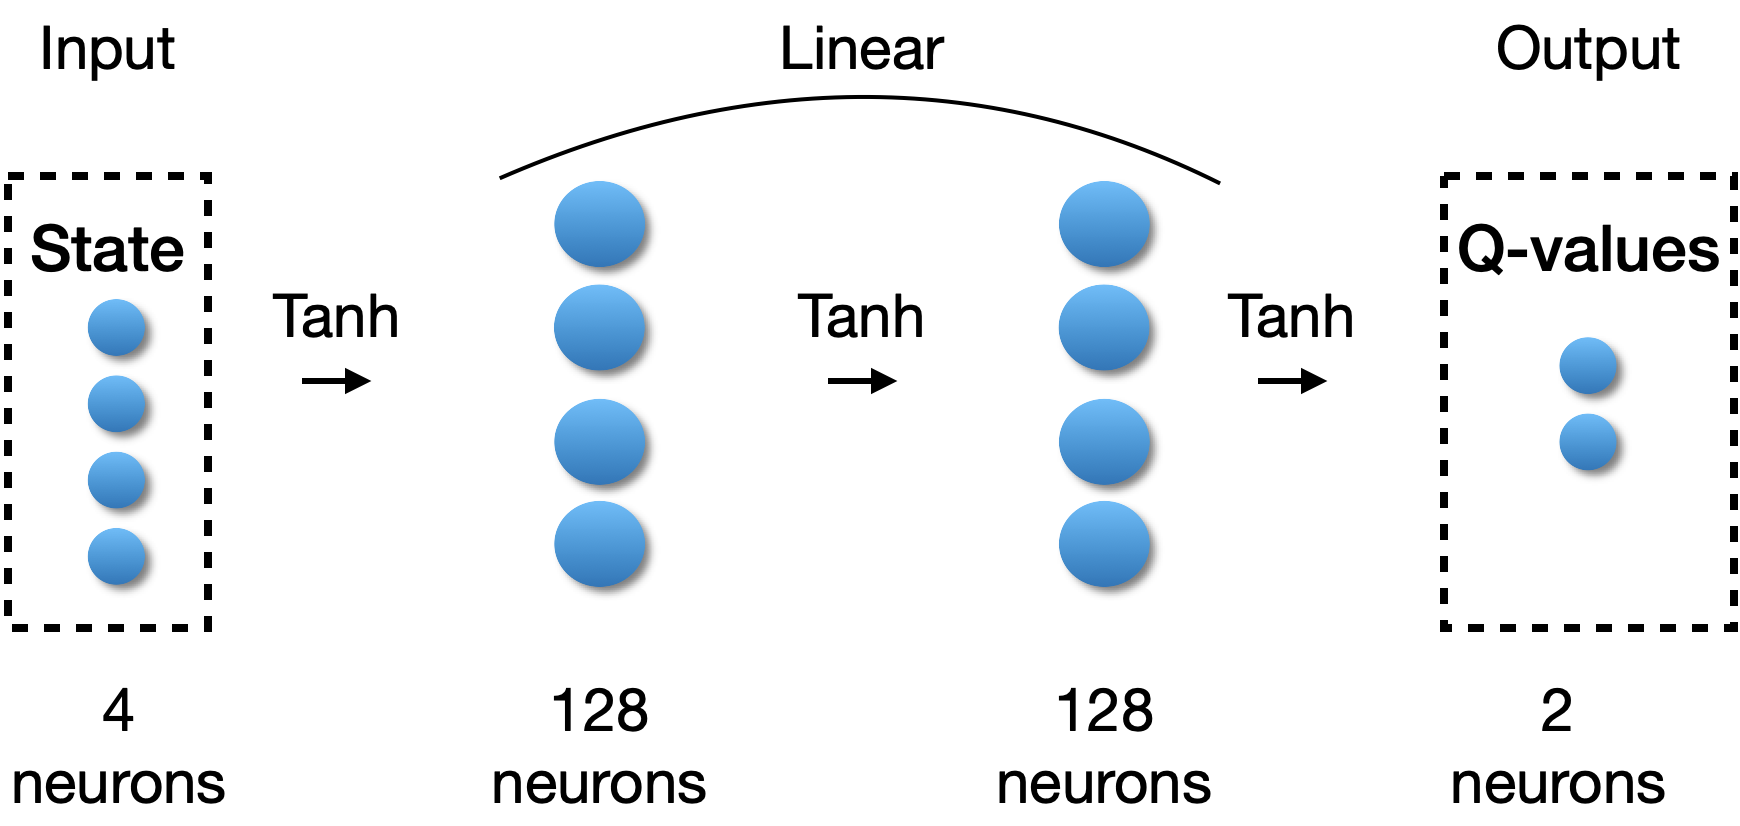
\includegraphics[width=0.6\textwidth]{Images/DQNet.png}
    \caption{Neural network for the evaluation of the $Q$-values given the state.}
    \label{fig:dqnet}
\end{figure}


In the reward function it is added a linear penalty proportional to the distance from the center of the screen, due to a problematic behavior of the agent that tried to "exit" 
from the screen.

We will try to speed up convergence as much as possible, in particular optimizing:
\begin{itemize}
    \item the exploration profile, of which we will change the starting temperature. As cited before, we will add gaussian increment of temperature at random position 
        in the profile with probability $p=0.3$, to understand its effect on the optimization. The exploration profile will be made of $1000$ points;
    \item The discount rate $\gamma$;
    \item The target update time $\tilde{n}$;
    \item The learning rate $\lambda$;
    \item The mini-batch size.
\end{itemize}

\subsection{Results}

We immediately understand that the performances of the algorithm are strongly dependent on the hyperparameters. We can see in Figure \ref{fig:hyper} the 
hyperparameter search, where the first\_solved axis is defined as the first time at which the agent performs at least $490$ points. If the agent is not able 
to solve the environment then we assign a first\_solved value of $1000$. We can see that the best performing agents have a high learning rate $\lambda$, a high 
discount rate $\gamma$ and a frequent update of the target network.
To better understand the evolution of the training and the effect of the exploration profile we plot the exploration profile and the training score, i.e. the score 
along all the points of the exploration. Obviously, they have different magnitudes, and so we will refer to the left axis for the exploration profile and to 
the right axis for the training score. The training score oscillates a lot along the evolution. We will so take an average each $20$ time step, taking as relative time step 
the central one. We see in Figure \ref{fig:best_cart} the best performing hyperparameters, in Figure \ref{fig:norm_cart} a good hyperparameter set and in Figure \ref{fig:bad_cart}
a set which is not able to solve the environment. The figures show clearly that, when the hyperparameter set is optimal, the score abruptly increases as soon as the 
temperature approaches zero, i.e. when the agent starts to choose the best action. This means that the learning is really fast. 
A bad choice can instead damage the learning so much that the agent is never able to solve the environment.